%UNIT 3: RATIONAL NUMBER OPERATIONS - WORKSHEET 0 (IN-CLASS INSTRUCTION)
\documentclass[12pt, letterpaper, fleqn]{article}

% ----------------------------------------------------------
% PACKAGES
% ----------------------------------------------------------
\usepackage{graphicx}
\usepackage{xcolor}
\usepackage[most]{tcolorbox}
\usepackage{amsmath, amssymb}
\usepackage{fancyhdr}
\usepackage[utf8]{inputenc}
\usepackage[T1]{fontenc}
\usepackage{enumitem}
\usepackage{geometry}
\usepackage{tikz}
\usepackage{needspace}
\usepackage{multicol}

\usetikzlibrary{arrows.meta, calc}

% ----------------------------------------------------------
% PAGE SETUP
% ----------------------------------------------------------
\usepackage{times}
\geometry{letterpaper, top=1.25in, bottom=1.25in, left=1in, right=1in}

% ----------------------------------------------------------
% HEADER / FOOTER
% ----------------------------------------------------------
\newcommand{\logowidth}{3cm}
\setlength{\headheight}{20pt}
\setlength{\footskip}{40pt}

\pagestyle{fancy}
\fancyhf{}
\fancyhead[C]{\small\bfseries Adding & Subtracting Rational Numbers}
\fancyfoot[L]{\raisebox{2pt}{
\includegraphics[width=\logowidth]{kss.png}}}
\fancyfoot[C]{\thepage}
\fancyfoot[R]{7.6.0}

\renewcommand{\footrulewidth}{0.2pt}

% ----------------------------------------------------------
% THEME COLOR
% ----------------------------------------------------------
\definecolor{customteal}{HTML}{2fbdb9}

% ----------------------------------------------------------
% HELPER MACROS
% ----------------------------------------------------------
\newcommand{\blank}{\underline{\hspace{2.2cm}}}
\newcommand{\blanklong}{\underline{\hspace{6.5cm}}}
\newcommand{\blankshorter}{\underline{\hspace{1.5cm}}}

% ----------------------------------------------------------
% DOCUMENT
% ----------------------------------------------------------
\begin{document}

\textbf{Name:} \underline{\hspace{5cm}}
\hfill
\textbf{Date:} \underline{\hspace{3cm}}\\

% ==========================================================
% SECTION 1: ADDING & SUBTRACTING RATIONAL NUMBERS
% ==========================================================
% --- PART A ---
\begin{tcolorbox}[colback=customteal!20]
\large\textcolor{black}{\textbf{Part A: Adding \& Subtracting Rational Numbers}}
\end{tcolorbox}

\vspace{3mm}

\begin{enumerate}[itemsep=2.2cm, leftmargin=0.6cm]
\item Always start at $0$.
\item Move \textbf{right} for positive numbers, and \textbf{left} for negative numbers.
\item Evaluate: $-\dfrac{3}{4} + \left(-\dfrac{1}{2}\right)$
\vspace{1cm}
\begin{itemize}
\end{enumerate}

\newpage

% --- PART B ---
\begin{tcolorbox}[colback=customteal!20]
\large\textcolor{black}{\textbf{Part B: Adding \& Subtracting Rational Numbers}}
\end{tcolorbox}

\vspace{3mm}

\begin{enumerate}[itemsep=2.2cm, leftmargin=0.6cm, resume]
\item Common Denominator Setup: \blanklong
    \vspace{0.5cm}
\item Final Answer: \blank
\end{itemize}
\item Evaluate: $-4.25 - (-1.5)$
\vspace{1cm}
\begin{itemize}
\end{enumerate}

\newpage

% --- PART C ---
\begin{tcolorbox}[colback=customteal!20]
\large\textcolor{black}{\textbf{Part C: Adding \& Subtracting Rational Numbers}}
\end{tcolorbox}

\vspace{3mm}

\begin{enumerate}[itemsep=2.2cm, leftmargin=0.6cm, resume]
\item Rewrite as Addition: \blanklong
    \vspace{0.5cm}
\item Final Answer: \blank
\end{itemize}
\item Model the expression $2 - 3.5$ on the number line below and find the final value.
\vspace{5mm}
\begin{center}
\begin{tikzpicture}[x=1.8cm, y=1cm]
  \draw[latex-latex, thick] (-3.5,0) -- (3.5,0);
  \foreach \x in {-3,-2,-1,0,1,2,3} {
    \draw (\x, 0.1) -- (\x, -0.1) node[below=2pt] {\small\x};
  }
  \foreach \x in {-2.5,-1.5,-0.5,0.5,1.5,2.5} {
    \draw (\x, 0.05) -- (\x, -0.05);
  }
\end{tikzpicture}
\end{center}
\vspace{0.5cm}
\begin{itemize}
\end{enumerate}

\newpage

% --- PART D ---
\begin{tcolorbox}[colback=customteal!20]
\large\textcolor{black}{\textbf{Part D: Adding \& Subtracting Rational Numbers}}
\end{tcolorbox}

\vspace{3mm}

\begin{enumerate}[itemsep=2.2cm, leftmargin=0.6cm, resume]
\item Final Answer: \blank
\end{itemize}
\item Represent the initial elevation as a negative decimal: $-45.5$
\item Represent the descent as subtracting a positive value or adding a negative value. Convert $20\dfrac{1}{4}$ to decimal: $20.25$
\item Set up the equation:
    \[
    -45.5 - 20.25 = -45.5 + (-20.25)
    \]
\item Add the absolute values and keep the negative sign:
    \[
    45.5 + 20.25 = 65.75 \implies -65.75
    \]
\end{enumerate}

\end{document}
